% Working manuscript based on Elsevier's elsarticle-template-num.tex.
% The unmodified upstream template and its license are in template/.
\documentclass[preprint,12pt]{elsarticle}

\usepackage[T1]{fontenc}
\usepackage{amsmath,amssymb}
\usepackage{booktabs}
\usepackage[hidelinks]{hyperref}

\journal{Chaos, Solitons \& Fractals}

\begin{document}
\begin{frontmatter}

\title{Working title}
\author{Authors to be added}
% Add author affiliations and the corresponding author's email here.

\begin{abstract}
\textit{To be written: motivation, method, principal results, and significance.}
\end{abstract}

\begin{keyword}
% Replace these draft keywords when the scope is agreed.
Astrocytes \sep Calcium dynamics \sep Piecewise affine models \sep NEST
\end{keyword}

\end{frontmatter}

\section{Introduction}
\label{sec:introduction}
% Motivation, related work, research question, and contributions.

\section{Model and methods}
\label{sec:methods}
% Reference model, approximation, solver, and validation protocols.

\begin{figure*}[tp]
  \centering
  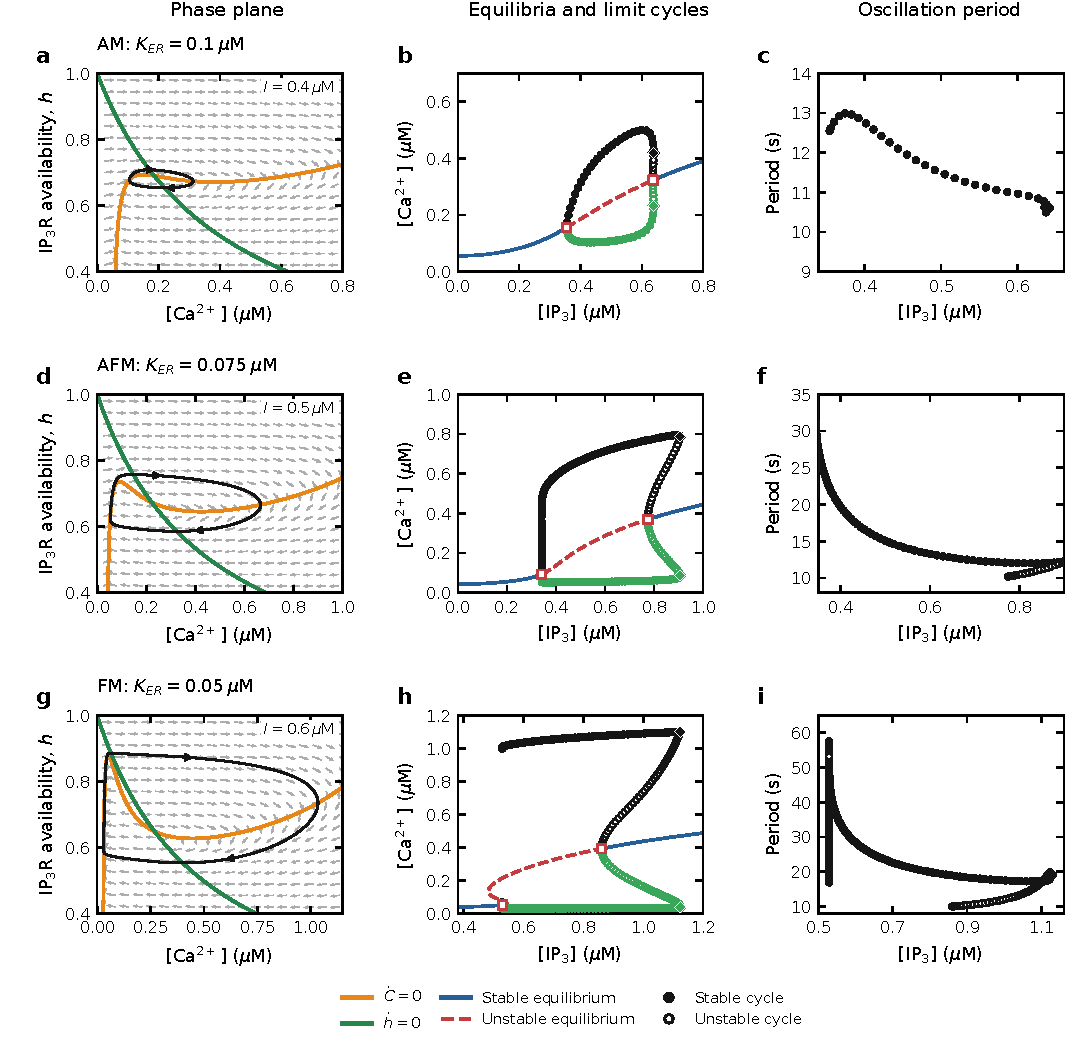
\includegraphics[width=\textwidth,height=.73\textheight,keepaspectratio]{figures/figure1_li_rinzel.pdf}
  \caption{Amplitude-, mixed amplitude--frequency-, and frequency-modulated calcium oscillations in the
  Li--Rinzel model~\cite{LiRinzel1994} at constant IP$_3$ concentration $I$.
  The panel organization follows Fig.~2 of De~Pitt\`a
  et~al.~\cite{DePitta2009}; all curves are computed independently from the
  nonlinear equations used in this work.
  \textbf{(a--c)} AM parameters, $K_{ER}=0.1\,\mu$M.
  \textbf{(d--f)} intermediate AFM parameters, $K_{ER}=0.075\,\mu$M.
  \textbf{(g--i)} FM parameters, $K_{ER}=0.05\,\mu$M.
  \textbf{(a,d,g)} Calcium nullcline $\dot C=0$ (orange), receptor-availability
  nullcline $\dot h=0$ (green), direction field (grey), and a stable limit cycle
  (black), at $I=0.4$, $0.5$ and $0.6\,\mu$M, respectively.
  Arrows indicate the direction of motion; field-arrow lengths are normalized
  in axis coordinates.
  \textbf{(b,e,h)} Stable equilibria (solid blue), unstable equilibria including
  saddles (dashed red), and calcium maxima (black) and minima (green) of
  periodic orbits. Filled and open circles denote stable and unstable cycles,
  respectively. Squares mark Hopf points; diamonds mark the upper folds of
  periodic orbits.
  \textbf{(c,f,i)} Periods of the same periodic orbits.
  Cycle stability is determined from the nontrivial Floquet multiplier.
  Near the lower FM boundary, continuation is truncated when an independent
  one-period integration no longer resolves closure to
  $2\times10^{-6}$ in $(C,h)$; the last displayed point is a numerical cutoff,
  not an identified global bifurcation.}
  \label{fig:li-rinzel}
\end{figure*}


\section{Results}
\label{sec:results}
% Add verified results and figures from the repository.

\section{Discussion}
\label{sec:discussion}
% Interpretation, limitations, and comparison with related methods.

\section{Conclusions}
\label{sec:conclusions}

% Complete these statements with the authors before submission.
\section*{CRediT authorship contribution statement}
\section*{Declaration of competing interest}
\section*{Acknowledgements}
\section*{Data availability}

\bibliographystyle{elsarticle-num}
\bibliography{references}

\end{document}
